\section{Validation}
\label{sec:validation}

Showing what algorithms should be implemented by the platform and 
defining the API will be part of our future work.  In this section
we provide evidence to support our conjecture.  We implemented
simple classifiers built using common pre-processing algorithms for
two accelerometer-based applications.  We evaluated the various sensing 
approaches using trace-based simulations.  We present recall and sleep time
metrics obtained from these simulations.



\begin{figure}[t]
\centering
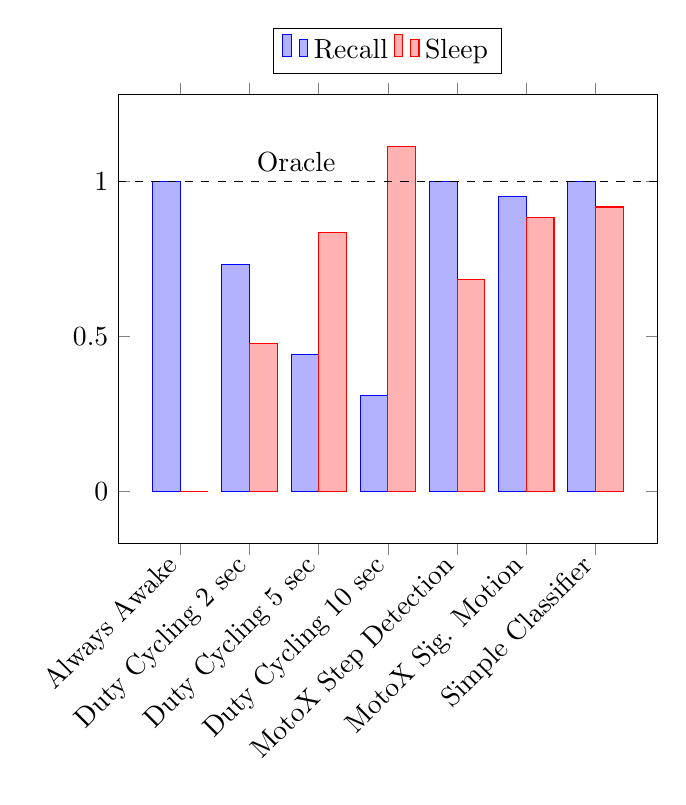
\begin{tikzpicture}
\begin{axis}[
	ybar=0pt,% space of 0pt between adjacent bars
	enlargelimits=0.15,
	legend style={at={(0.5,1.15)},anchor=north,legend columns=-1},
	symbolic x coords={
		Always Awake,
		Duty Cycling 2 sec,
		Duty Cycling 5 sec,
		Duty Cycling 10 sec,
		MotoX Step Detection,
		MotoX Sig. Motion,
		Simple Classifier},
	x tick label style={rotate=45,anchor=east},
	xtick=data,
	%nodes near coords,
	nodes near coords align={vertical},
]
\addplot coordinates {
	(Always Awake,1.0) 
	(Duty Cycling 2 sec,0.73) 
	(Duty Cycling 5 sec,0.44) 
	(Duty Cycling 10 sec,0.31)
	(MotoX Step Detection, 1.0)
	(MotoX Sig. Motion, 0.95)
	(Simple Classifier, 1.0)};
\addplot coordinates {
	(Always Awake,0.0) 
	(Duty Cycling 2 sec,0.476667) 
	(Duty Cycling 5 sec,0.833333) 
	(Duty Cycling 10 sec,1.111111) 
	(MotoX Step Detection, 0.683)
	(MotoX Sig. Motion, 0.883333)
	(Simple Classifier, 0.916667)};
\draw [black, dashed] ({rel axis cs:0,0}|-{axis cs:Always Awake,1}) -- ({rel axis cs:1,0}|-{axis cs:Always Awake,1}) node [pos=0.33, above] {Oracle};
\legend{Recall,Sleep}
\end{axis}
\end{tikzpicture}
\caption{Footstep Detection}
\label{table:footstepDetectionRecallSleepTime}
\end{figure}


\begin{figure}[t]
\centering
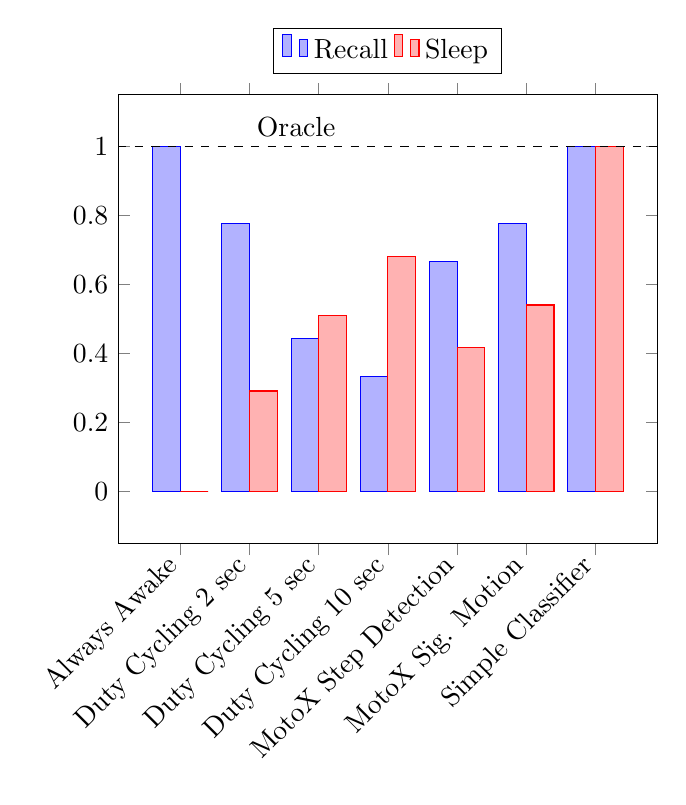
\begin{tikzpicture}
\begin{axis}[
	ybar=0pt,% space of 0pt between adjacent bars
	enlargelimits=0.15,
	legend style={at={(0.5,1.15)},anchor=north,legend columns=-1},
	symbolic x coords={
		Always Awake,
		Duty Cycling 2 sec,
		Duty Cycling 5 sec,
		Duty Cycling 10 sec,
		MotoX Step Detection,
		MotoX Sig. Motion,
		Simple Classifier},
	x tick label style={rotate=45,anchor=east},
	xtick=data,
	%nodes near coords,
	nodes near coords align={vertical},
]
\addplot coordinates {
	(Always Awake,1) 
	(Duty Cycling 2 sec,0.7778) 
	(Duty Cycling 5 sec,0.4444) 
	(Duty Cycling 10 sec,0.3333) 
	(MotoX Step Detection,0.6667)
	(MotoX Sig. Motion, 0.7778)
	(Simple Classifier, 1)};
\addplot coordinates {
	(Always Awake,0.0) 
	(Duty Cycling 2 sec,0.291545) 
	(Duty Cycling 5 sec,0.510204) 
	(Duty Cycling 10 sec,0.680272) 
	(MotoX Step Detection, 0.418367)
	(MotoX Sig. Motion, 0.540816)
	(Simple Classifier, 1)};
\draw [black, dashed] ({rel axis cs:0,0}|-{axis cs:Always Awake,1}) -- ({rel axis cs:1,0}|-{axis cs:Always Awake,1}) node [pos=0.33, above] {Oracle};
\legend{Recall,Sleep}
\end{axis}
\end{tikzpicture}
\caption{Fall Detection}
\label{table:fallDetectionRecallSleepTime}
\end{figure}

\vspace{3 mm}

This section:

\begin{enumerate}
\setlength{\itemsep}{-3pt}  

\item Highlights the limitations of the Duty Cycling and Batching approaches

\item Illustrates the inflexibility of Predefined Event detection featured by current
  generation smartphones
  
\item Demonstrates that simple classifiers built from common pre-processing algorithms
can achieve close to ideal recall and device sleep time

\end{enumerate}

\subsection{Trace Collection}

We collected two traces from human subjects using a Motorola Moto X device, running Android 4.4.4.
The smartphone ran an application that kept the device always awake and 
continuously recorded all accelerometer readings and predefined event 
(significant motion and steps).

The first trace is about 10 minutes long and contains a combination of frequent events of interest
(steps; about 40\% of the trace) and infrequent events of interests (falls; about 2\% of the trace). 
We annotated this trace with ground truth information about the time stamps when events of interest
occurred.

The second trace is 2 hours and 50 minutes long representing a person's morning routine 
(getting ready, having breakfast and commuting to work). This trace was not annotated with ground truth
information.

\subsection{Applications}
\label{sec:applications}

We developed two applications that detect activities performed by 
human subjects:

\begin{enumerate}
\setlength{\itemsep}{-3pt}  

\item A {\em Step Detector} based on the human step detection algorithm
  proposed by Ryan Libby in~\cite{libbyFootstepDetection}.

\item A {\em Fall Detector} based on a simple thresholding algorithm, as
  described in~\cite{kangasFallDetection}.

\end{enumerate}


\subsection{Simple classifiers}
\label{sec:classifiers}

We created {\em simple classifiers} for our step and fall
detection applications. 

\vspace{3 mm}
The step detection classifier consisted of:

\begin{enumerate}
\setlength{\itemsep}{-3pt}  

\item A {\em noise-reduction} step, based on exponential moving average.

\item A {\em feature extraction} step, computing the magnitude of the noise-reduced
  acceleration vector.
  
\item An {\em admission control} step, checking if the total acceleration magnitude
  exceeds a threshold.

\end{enumerate}

The fall detector classifier was similar, with the following differences:

\begin{enumerate}
\setlength{\itemsep}{-3pt}  

\item The {\em noise-reduction} step was milder, resulting in more detailed accelerometer data.

\item There were two {\em admission control} steps.  It checks for acceleration magnitude 
  below a small threshold (representing free-fall), followed by a spike in acceleration magnitude 
  above a different threshold (representing the moment of impact).

\end{enumerate}

\subsection{Oracle}

A hypothetical ideal implementation that only wakes up
when an event of interest occurs.  Such a wake-up condition would
achieve perfect precision\footnote{$$Precision=\frac{True Positives}{(True Positives + False Positives)}$$}
and recall\footnote{$$Recall=\frac{True Positives}{(True Positives + False Negatives)}$$}, with
the highest possible sleep time. The difference between the
power consumption of this method and our approach
provides an upper bound on the potential additional benefits of custom
code offloading.

This setup provides a baseline for comparison. Figures~\ref{table:footstepDetectionRecallSleepTime} 
and~\ref{table:fallDetectionRecallSleepTime} show the event of interest recall and achieved sleep time
for various sensing approaches, normalized by the recall and sleep time of the {\em Oracle}. 
We assumed that the Oracle achieves 100\% recall for both activities and sleeps for 60\% and 98\% of
the time for step detection and fall detection, respectively.

\subsection{Always Awake} 

The applications keep the phone awake all the time, constantly collecting accelerometer readings.  Under 
this sensing approach, both the step and fall detector applications
achieved very high levels of precision and recall for the 10 minute trace. The recall 
and precision achieved by the {\em Step Detector} were 100\% and 98\%, respectively. The {\em Fall Detector}
had perfect precision and recall.


\subsection{Duty Cycling} 

We modified the applications so that they check
sensor readings periodically and then put the phone to sleep.  On
wake-up, the phone is kept awake for 5 seconds in order to collect
sensor data.  This software-only implementation can run on any mobile 
device and does not require special hardware support. As expected, Duty Cycling is effective at reducing
the amount of time the device is awake (and thus, power consumption), but performs poorly in terms
of event of interest recall.



\subsection{Batching} 

This configuration emulates hardware support
available on the Nexus 5 and recent iPhone devices for collecting and batching accelerometer
readings while the main processor sleeps.  The application wakes up
periodically, reads the batch of sensor readings, runs the detection
algorithm(s), and goes back to sleep. Because the applications get access to all the sensor
data, their event of interest recall would be the same as the Always Awake approach. However, 
the power efficiency of this approach is dependent on 
several device-specific characteristics. The size of the sensor data buffer creates an upper bound
on the amount of time the device can be asleep, while ensuring that the application will 
eventually receive all the sensor data. The device's computational capabilities will have 
an impact on the amount of time it takes to process the data in a batch, and thus, the amount
of time the device needs to be awake. 

Batching is not appropriate for applications with timeliness
constraints.  For example, the user of a gesture recognition
application~\cite{liu2009uwave,schlomer2008gesture} would not be
satisfied if the application detects the performed gesture after a
delay of more than a couple of seconds. Additionally, the device would often wake up to find that no 
events have occurred in the current batch. We therefore conclude that 
batching will result in significant energy waste for applications 
interested in low frequency events (e.g., gesture recognition, fall 
detection).

\subsection{Predefined Event Detection} 

This configuration makes use of the features available in Android 4.4+ and iOS 
7.0+ for recognizing a limited number of predefined activities (significant motion 
and steps). 

We compared the ground truth annotations with the step events detected by the Android framework. 
The step detector achieved perfect recall, however, its precision was approximately
70\%. Upon inspection, we noticed that falls and other events such as sitting, standing and taking the
device out of the pocket were incorrectly classified as steps. The lack of configuration options available
in Android's sensor manager makes it impossible to calibrate the step detector for usage by specific users. 
As such, an application that requires high degrees of precision and recall would need to implement its own
step detection algorithm.

We wanted to see if the significant motion events detected by the device could be used as wake-up 
conditions for either step or fall detection, effectively removing the need for simple classifiers running
on a low-power processor.  From a recall point of view, significant motion
events were detected for nearly all the events of interest.  However, these events were delivered to the
application up to 10 seconds after the event occurred.  Without access to past sensor data, the
application is unable to determine if the activity that caused the significant motion event is indeed 
an event of interest.  Unless combined with sensor data batching, these
significant motion events would be useless for the application. 

To determine the feasibility of the significant motion event as a wake-up condition for events of
interest that occur infrequently, we analysed the 2 hour and 50 minute long trace. We assumed the event of interest
(e.g., falls) did not occur during the entire length of the trace. For this trace, the significant motion event
fired, on average, every 2.47 seconds. Using the significant motion event as a wake-up condition for infrequent
events of interest would be very inefficient from a power consumption perspective. The device would wake up too
frequently, without actually detecting any events of interest.

\subsection{Simple Classifiers} 

We defined simple classifiers to act as custom wake-up 
conditions as described in Section~\ref{sec:classifiers}. On
wake-up, the applications acquire the raw sensor readings used by the
classifier to detect the event and run their own detection algorithm, and go back to sleep.

Figures~\ref{table:footstepDetectionRecallSleepTime} and~\ref{table:fallDetectionRecallSleepTime} 
show that this approach achieved perfect recall of both events of interest. The difference in sleep time
between this approach and {\em Oracle} is attributed to unnecessary wake-ups resulting form false positives 
generated by the simple classifier. These false negatives were discarded by the detection algorithms 
implemented in the applications. 

\subsection{Limitations}

Establishing a greater support for the proposed conjecture requires a significantly more 
thorough evaluation. Additional traces need to be collected in order to increase certainty that the simple
classifiers we implemented significantly increase device sleep time, while maintaining event of interest
recall. The classifiers we constructed may be over-fitting to the trace used in the simulations. Moreover, 
simple classifiers would need to be constructed for a wider-range of accelerometer-based applications.


 